\chapter{La posición tecnocrítica es la destitución del Imperio}
\label{cha:la-posición-tecnocrítica-es-la-destitución-del-imperio}

De Laurentis prefiere el termino tecnología al de género para referirse a las formas de opresión performativas y moleculares que condicionan a las formas de vida a sus roles en la jerarquía social \autocite{preciadoTestoYonqui2008}. En este capítulo tomaremos una aproximación similar, al señalar la violencia desde los procesos tecnológicos que la producen considerando también una aproximación interseccional que parece reificar las subjetividades en procesos descriptivos donde las relaciones de género, de clase, raciales o coloniales ejercen el mayor poder descriptivo para analizar las formas de opresión. Si hasta el momento he tratado de explicar algunos componentes generales de la religión de Estado, en este capítulo analizare la cuestión de la guerra civil y la violencia desde sus tecnologías con la intención de proponer una alternativa al Estado moderno que al mismo tiempo sea capaz de responder al problema que según Tiqqun da origen al Estado, que es la guerra de religiones. Si decidí abordar la neorreaccion ha sido porque la cultura de blancos (\emph{whiteness}) profesa el nihilismo pero también posee el estatus de los agentes del Estado. Son propietarios, banqueros o patrones condenados a la misma cultura de hombre-masa que imponen a las personas que trabajan para ellos. En el vocabulario hacker se llama \emph{white hat} o sombrero blanco a los sujetos que practican el hacking, es decir, la intrusion o modificacion de codigos, con fines corporativos o legales. Podríamos decir que son los agentes del Estado con capacidad para desempeñar un papel propio más allá de la norma de su propia jerarquía. Es decir, aquellos con la capacidad de asumir una personalidad más allá de sus condicionamientos performativos y moleculares. Paradójicamente, son también aquellos que a partir del reconocimiento de su nihilismo son capaces de conjurar un afuera a la dominación mercantil por su posición tecnomaterial en la \emph{societas}. En este momento de la Historia tenemos lo necesario para implementar una economía pos-escasez. Se trata de intervenir estratégicamente en esas redes de información, que también son flujos de sentido, producciones de deseo. La utopía robótica tecnocapitalista es una de las aristas de distintos escenarios posibles planteados en Four Futures, donde señala que viviremos en un mundo materialmente condicionado por dos aristas, una de igualitarismo-estamentalismo (o sea, donde las jerarquías manden) y otra de abundancia (por la automatización tecnológica) o escasez (por nuevas formas de los patrones para crear valor explotable). De esos casos, los más extremos parecen ser el mundo donde quepan todos los mundos, sostenido por una infraestructura tecnológica común, y el exterminio, la utopía tecnocapitalista para 1~\% de la población global.

Las cuestiones estructurales afectan por una cuestión de origen, de diseño, sobre las tecnologías que configuran nuestra realidad. El capitalismo, objeto vacío, sustantivo que, al no tener una sustancia definida, concreta y subjetiva, se toma por la derecha como algo que no existe materialmente, sí existe y es un espectro psíquico. Para entenderlo, tenemos que comprender las diferencias entre Estado y Capitalismo en la historia y cómo funciona a grandes rasgos el panorama político a partir de estas diferencias. Sin embargo, el pensamiento del estatus quo es realmente poderoso en cuanto a que el Estado dispone de manera muy particular de los objetos como armas y herramientas que reproducen el modo de producción capitalista.

La capacidad del Espectáculo contemporáneo de producir deseos es extremadamente sutil pero molecularmente brutal. Se combina con el Biopoder, que es molar y molecular, configura su propia ecología a partir de cosas y de deseos. Estas performatividades son tan evidentes que, en términos de género, la forma patriarcal del Espectáculo condiciona al hombre al Bloom y a la mujer a actuar como la princesa a ser salvada.\footnote{Tiqqun intenta hacer un análisis de esta condición opuesta al Bloom en \autocite{PrimerosMaterialesPara}. Recomiendo ver la serie de conversatorios de Leonor Silvestri titulados Teoría de la mala víctima.} Hoy en día, la cuestión se trata de una agresiva campaña por captar la atención de las personas para enganchar sus deseos \autocite{fernandez-savaterAusentarseCrisisAtencion, lanhamEconomicsAttentionStyle2007}. La industria cultural de internet o FAAMG, es decir, Facebook, Amazon, Apple, Microsoft y Google, invierten millones de dólares para programar micropolíticas de género, comportamientos y sustancias, es decir, son artífices de un proyecto capitalista de construcción de subjetividad. En el siguiente apartado trataré de plantear qué sentido tendría un Partido en tiempos donde los mecanismos del Imperio operan con toda libertad y sin que nadie pueda detenerlos \autocite[p.~52]{comiteinvisibleAhora2017}.

\section{Un Partido sólo tiene sentido si conduce a la destitución del Imperio}
\label{sec:un-partido-sólo-tiene-sentido-si}

\epigraph{La guerra es la eventualidad suprema.}{\emph{El Comité Invisible} en~\autocite{comiteinvisibleTeoriaBloom}.}

\subsection{El Partido imaginario se constituye del Bloom}
\label{sub:el-partido-imaginario-se-constituye-del-bloom}

Este apartado es un análisis centrado en las Tesis sobre el Partido imaginario. De acuerdo con Tiqqun, el Partido imaginario es la forma de la Contradicción en la dictadura de y en la visibilidad. Es decir, del Espectáculo. El Espectáculo hace invisible la negación. Se compone de la multitud negativa de los que no tienen clase y no la quieren tener, de la no-pertenencia a la sociedad mercantil. En lo que respecta a la relación entre el Partido imaginario y el Espectáculo, la multitud de clase se configura del siguiente modo: el Espectáculo y el Biopoder buscan apoderarse de todo a través de la lógica de la representación. Busca romper la posibilidad de un afuera y recurre a cualquier ficción, como la Jovencita. Desde el punto de vista del PI, la ciudadanía es la dictadura del deber abstracto de participación en una totalidad social atomizada. La multitud de los indiferentes se vuelve entonces multitud de las personas rebeldes, \emph{Waldgänger}. En el Éxodo se dibujan sentimientos que hacen que la oposición formal entre Espectáculo y PI se vuelva concreta \autocite{tiqqunTesisSobrePartido}. De lo marginal esencial se genera una pertenencia a la no-pertenencia, una comunidad del exilio. La fuga se vuelve estrategia, la política suprema. No existe crisis sino la omnipresencia del P.I., que no tiene centro ni circunferencia pues opera en el mismo territorio que el Espectáculo. La amenaza del Espectáculo no es otra cosa más que sus artífices y trabajadores alienados. Hombres sin aliento, que se juran mutuamente igualdad y respeto pero profesar un profundo deseo por escapar a todo.

El \emph{Waldgänger},\footnote{Este concepto está basado en la obra \emph{Eumeswill} de Ernst Jünger, donde desarrolla el perfil del \emph{anarca}, que se distingue del anarquista por su carácter radicalmente solitario y escéptico \autocite{jungerEumeswil2011}. } aquel que se descubre viviendo en el bosque de sí mismo y es capaz entonces de recuperar la soberanía sobre sí, es una de las formas del Bloom, que hoy en día se encuentra más dispuesto a la destitución pues ha sido expurgado de la sociedad y en su nihilismo, es incapaz de participar del arreglo mercantil. Los neorreaccionarios son el momento en que el Bloom toma partido por el resentimiento y por el nihilismo, para hacer reales y concretos el tanatos que despierta en ellos la alienación mercantil y el rechazo social por resistirse a participar del deseo social. Como la frase de un gangsta en Ocuppy Wall Street

\begin{quote}
  \enquote{Hi! What' s up? My name is Mike. I'm just a gangster from Harlem. I hate my life. Fuck my boss! Fuck my girlfriend! Fuck the cops! I just wanted to say: I'm happy to be here, with you all.} \autocite{comiteinvisibleNuestrosAmigos2015}
\end{quote}

La política masculina reproduce un modelo de activismo \emph{Choose your Own Adventure}. Es la cualidad del héroe, del Ulises desesperanzado porque sus deseos de gobernar han sido aplacados por los sillones de diseño o el espacio público diseñado para alejar a la gente de la calle, por una civilidad autoimpuesta. El Bloom es en realidad el más \emph{sujeto} al Estado, es quien da sentido al mito del Héroe, a la construcción de una Gran Historia Universal o de Una Gran Conciencia. Lo que en \emph{Introducción a la Guerra civil} denominan como la necesidad del Uno, de Dios, de la Razón, de La Ciencia. En las \emph{Tesis sobre el Partido imaginario}, el Comité Invisible menciona que el Biopoder es un momento del Espectáculo. El Espectáculo tiene que ocultar la violencia que implica reconocer que su proyecto es un proyecto meramente metafísico. No se reconoce por el temor que el Espectáculo tiene al vacío. El Espectáculo tiene una campaña de pacificación de las sociedades y de neutralización de sus contradicciones. Su campaña de pacificación es todavía una guerra, pero se reemplaza el tema de la guerra en el lenguaje. Se habla, ante todo, de \enquote{procesos de paz}. En mis palabras, la tesis ocho señala que masas de hombres silenciosos se preparan para el éxodo, rechazan participar en todo lo que tiene que ver con el mundo mercantil. Se dibuja un ethos, un mundo infraespectacular que parece un crepúsculo pero es en realidad un alba, parece una experiencia masiva de la ilegalidad y la clandestinidad. El ocaso compuesto de parches es el espectáculo grandioso y mortal que se devela a quien se atreve a considerar su tiempo desde el punto de vista de su negación, es decir, desde el punto de vista del Partido Imaginario. La noción del PI vuelve visible la nueva configuración de las hostilidades; reivindica lo que conspira por la destrucción del orden presente y el desastre es su obra. El PI es el espectro de lo otro, en una sociedad donde la alteridad ha sido suprimida, es el otro nombre de la paranoia, de la enfermedad de los poderes. En el Imperio como fase terminal del Estado moderno, éste no habla más que de terrorismo, delincuencia, criminalidad, pero nunca del PI. \autocite{tiqqunTesisSobrePartido}.

El estado actual de los Bloom es la toma de Partido por una forma de terrorismo organizada que tiene por objeto hacer efectiva una sociedad donde el otro es plenamente un objeto. El nihilismo espiritual del Bloom es también una condición psíquica caracterizada por la marginalidad y la completa desconexión entre mente y cuerpo, el síntoma de la no-sexuación del hombre blanco heterosexual, de la cual los \emph{incels} (\emph{involuntary celibates}) son el principal exponente. La comunidad de célibes involuntarios son el caso extremo de un estado de resentimiento, frustración y de mala conciencia frente a las mujeres y al feminismo en general por ser una militancia en contra de la objetivación sexual de la mujer ---y del otro en sus diferentes formas. Se trata de comunidades de hombres militantes contra el feminismo y que construyen espacios de odio contra cualquier forma de vida distinta, pues el mero hecho de su existencia representa la arbitrariedad de la metafísica de la nada propia del Bloom. En el artículo de Villodres señalan que convertir a \enquote{la otra} en algo objetual e identificarla como un \enquote{no yo/no igual a mí} es un un pensamiento común entre las personas reaccionarias y fanáticas \autocite{villodresQueSonIncels2018}. Yo añadiría que esta disposición reaccionaria no solo construye a la otra como un objeto en términos de género, sino que construye a toda diferencia como un objeto frente al cual es \emph{deber} adoptar una postura hostil.

Sin embargo, la fuerza espiritual y sexual del Bloom tiene alternativas más allá de la neorreacción como partido del resentimiento (cuya agenda es el totalitarismo urbano tecnocapitalista). La guerra contra la dominación mercantil y contra la religión de Estado solo podrá encontrar victorias allí donde la acción se dirija a la disolución misma del que es/tá \emph{sujeto}, a la \emph{destitución} tecnomaterial del estado actual de las cosas. Una toma de partido por una acción libertaria, tecnocrítica.

\begin{figure}
  \centering
  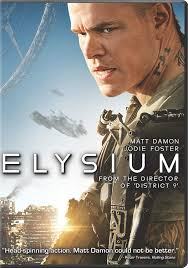
\includegraphics[width=0.7\linewidth]{images/elysium.png}
  \caption{Cartel de la película Elysium, que muestra una tecnoutopía lunar semejante al escenario de exterminio descrito en \emph{Four Futures}.}
  \label{fig:elyssium}
\end{figure}

\subsubsection{¿Una hegemonía del sentido común?}
\label{una-hegemonía-del-sentido-común}

Hardt y Negri señalan que participamos en un momento más radical y profundamente comunal que nunca en la historia del capitalismo, produciendo medios de cooperación y comunalidades comunicativas gracias a la interconexión global producida por internet. El negrismo tiene la esperanza de un Estado democrático mundial. Para el Comité Invisible, sus seguidoras se comportan como si no entendieran que dentro de los edificios pomposos frente a los que acampan no hay realmente nada. Toda la visión negrista se encarga de forzar al Imperio, a través de la emergencia de una supuesta \enquote{sociedad civil mundial}, a darle la forma a un Estado universal. Que esto no nos engañe, señalan. Si bien el Imperio tiene una fachada institucional, su realidad efectiva permanece concentrada en la policía y la publicidad mundiales, que por sus capacidades son ya Biopoder y Espectáculo \autocite{comiteinvisibleNuestrosAmigos2015}. Las intervenciones militares de los países progresistas no son el avance de un derecho mundial naciente sino la subordinación del orden jurídico al estado de excepción policial. Frente a ello, resulta más fructífero devastar al Espectáculo y al Biopoder que militar en favor de un Estado universal salvador.

Diré algo para provocar a las personas afines a la teoría populista que pugna por la hegemonía del \enquote{sentido común}: si recordamos que el Partido imaginario es el motín, siempre presente, del proletariado global y que su existencia evidencia, junto con el cinismo, la fragilidad de los planteamientos que dan forma al Estado moderno, la dialéctica entre constituyente y destituyente es un falso dilema, pues ambas forman parte de una dialéctica de la acción, una tensión entre dos formas de \emph{praxis}. Además del sentido común como lo plantearían Laclau y Mouffe \autocite{laclauRazonPopulista2016}, también se trata de una hegemonía tecnomaterial, como lo han defendido Srnicek, Williams y Hester [@\autocite{hesterXenofeminism2018}] . Para mí, las posibilidades de la acción crítica apuntarían a una pragmática \emph{Free Libre Open Source Software (FLOSS)}, una etiqueta que en la jerga de programación se refiere a la creación de códigos completamente abiertos, manipulables y anticapitalistas. Mientras que la tecnocrítica se ocuparía del develamiento de los dispositivos de poder y al diseño de un porvenir poseconómico.

\subsection{¿Necesitamos más manifiestos políticos?}
\label{necesitamos-muxe1s-manifiestos-políticos}

Al analizar los manifiestos de Maquiavelo y de Marx y Engels, Hardt y Negri señalan que todo manifiesto político efectivo se posiciona sobre un sujeto, que para ellos es la multitud, y un objeto, la liberación cosmopolita dentro del abismo de la posmodernidad \autocite[p.~64]{hardtImperio2005}. Al respecto, considero que las formas de vida configuran el mundo a través de su deseo y de su capacidad de accionar para hacerlo efectivo. Hay que analizar \enquote{la multitud} y la \enquote{liberación cosmopolita}, es decir, determinar un sujeto que acciona.\footnote{Que para mí sería algo así como las formas de vida se posicionan por una areté tecnocrítica.} Analicemos un poco estas posibilidades en medio del debate sobre el Partido y el poder constituyente.

En primer lugar, la multitud es un sujeto social activo que parte de lo común, de las singularidades. No se funda en la identidad, ni en la unidad sino en lo que hay en común \autocite[p.~128]{straehleDIFICULTADESMULTITUDDISCUSION}. Está opuesta a la soberanía, propugna por horizontalidad, es el ensamble de lo singular en lo colectivo sin desembocar en una abstracción genera. De igual modo niega los flujos de poder. Son singularidades que abolen la identidad, no son individuos \autocite{hardtMultitudGuerraDemocracia2006}. Esto emerge gracias a los procesos sociales colaborativos de la producción. Se pasa de la \emph{res pública} a la \emph{res communis}, plantean la asunción de un interés o voluntad general. Esto para alcanzar una libertad más allá de las identidades. Esta subjetividad política está en respuesta al trabajo inmaterial (posfordismo) en una época donde el capitalismo evoluciona a capitalismo cognitivo. La incorporación de la multitud a la política es indeseable pero necesaria. Su concepto de multitud viene de Spinoza. Hardt y Negri argumentan que la multitud no es un concepto sino una realidad nueva. La apología de la multitud conlleva el deseo de que la realidad adopte los flujos históricos del capitalismo como respuesta política. Se prescribe el síntoma como la estrategia última. La multitud está encerrada en una política de mínimos, de un denominador común irrebasable, que alcanza resultados para la unión en la protesta pero no en la construcción.

El problema de la multitud es su indefinición. No se puede saber la orientación que tomará este grupo, o que reproduzca la fuerza capitalista, esa es la cuestión que trae a colación Žižek al preguntar:

\begin{quote}
  \enquote{¿Qué haría este proclamado nuevo sujeto, \enquote{la multitud}, una vez en el poder? ¿Cómo funcionaría el movimiento antiglobalizador reunido en Porto Alegre, ese conjunto de agencias y posiciones políticas incompatibles entre sí? ¿Cómo podrían convivir los granjeros que reclaman proteccionismo con los grupos de derechos humanos y los representantes de los intereses de los inmigrantes que pelean por una mayor movilidad global? Esta lógica de multitud funciona porque estamos hablando de resistencia. Sin embargo, ¿qué pasa cuando \enquote{tomamos el poder}? --si es que éste es realmente el deseo y la voluntad de estos movimientos--. ¿Qué sería una multitud en el poder?}~\autocite{zizekRevolucionBlanda2004}.
\end{quote}

La cuestión es que la multitud solo se define como negatividad a algo. Tiene una tendencia igualmente reaccionaria que parece ignorar las capacidades del poder contrarrevolucionario del Imperio. La multitud fracasa por la tiranía de la no-estructura @TyrannyStucturelessness, pues la potencia para lo común es distinta a la potencia de lo común. Es decir, una multitud que reacciona hacia un \emph{interés común} no es lo mismo que la producción deseante en comunidad y en ese sentido, la multitud carga en su génesis, el interés común, el origen de toda \emph{societas}, de todo contrato social moderno. El concepto de multitud abarca a todos aquellos cuerpos políticos que desde afuera demandan soberanía sobre dispositivos que el Estado ha reservado para sí en cuanto órgano que monopoliza la violencia. Estas multitudes son identidades políticas rizomáticas y solo por poseer esta característica representan una amenaza para el Estado: su hábitat es la heterotopía foucaultiana.

Hay una multitud, constituida realmente como clase, cuya potencia nuclear representa la amenaza más peligrosa para el Estado: la multitud de lxs nadie. Si, como lo señala el Comité Invisible, la economía, la cibernética y la inteligencia son las nuevas bases del Estado como control, el Partido imaginario representa la amenaza más terrible por una razón: el capitalismo basa su dominación sobre el mundo a través de la métrica, de la categorización total del mundo, y el grado absurdo de improvisación, la pureza que proviene de una ausencia de necesidad y de deseo, convierte a estas formas de vida en latencias tan inestables que podrían, de un momento a otro, contaminar cada circuito de este gran sistema complejo de La Necesidad \autocite{EconomiaConsideradaComo}. Todas aquellas formas-de-vida que puedan constituirse de tal modo que su puesta en escena muestre al otro la facilidad de destituir el mundo a través del acto creativo, serán aliadas silenciosas de lo que Tiqqun denomina el Partido imaginario. La multitud, cuya configuración siempre es en torno a una identidad, es un nodo abstracto y su salvación está solo en su capacidad de reconquistar el territorio que, quizá sin saberlo, habita en el imaginario. En la tesis VII señalan que el Partido imaginario es el partido de lo político, toma como foco de la sociedad el trabajo metafísico de una hostilidad absoluta. Por tanto, toma el camino de la \enquote{política absoluta}. Es la forma de lo político en el colapso de los Estados-nación, donde lo político es el elemento total, existencial, metafísico, en el cual se mueve la libertad humana.

Incluso la multitud como subjetividad parece ser otro alcahuete del estado de las cosas. Citando al Comité Invisible: \enquote{El liberalismo existencia ha propagado tan bien su desierto que al final hasta los izquierdistas más sinceros enuncian sus utopías usando sus mismos términos.} \autocite[p.~23]{LlamamientoOtrosFogonazos2009}. Siguiendo a los aceleracionistas de izquierda, creo que ni la Ilustración ni el progreso tienen significados definitivos. Todo el tiempo se constituyen como conceptos en disputa y sobre los motivos de su apropación debería tratar un manifiesto político contemporáneo. Es necesario, en principio, recuperar un concepto de la libertad. Srnicek y Williams insisten en pugnar por la libertad sintética, que es libertad para, potencia y capacidad de acción \autocite{srnicekInventarFuturoPoscapitalismo2017}. Yo añadiría que al mismo tiempo que es libertad-para, es liberación-del yo, del ego, del sujeto. Para mí, la libertad es en parte la renuncia, la deserción a la máquina social de producción deseante y de la economía que sostiene la explotación planetaria de las formas de vida.

En lo que respecta a los temas, habría que imaginar un manifiesto político al alcance de la \emph{complejidad} de nuestros tiempos. Rescatando las enseñanzas de Haraway y de Preciado sobre la construcción molecular del género y las tecnologías de dominación, todo manifiesto, político o no, debería comenzar por situarse. A mi parecer, los planteamientos del Partido y el Poder constituyente tienen, por un lado, el optimismo de los dúos dinámicos Hardt-Negri y Srnicek-Williams, y algo que recuerda a la disputa por el sentido común de Mouffe para ganar los conceptos de universalismo y darles un sentido de libertad positiva, s\autocite{srnicekInventarFuturoPoscapitalismo2017}, libertad-para.

Creo que todo manifiesto político debería posicionarse también frente a los problemas económicos que dan origen a la dominación mercantil. Entre los retos del futuro también se encuentra el hackeo y destitución de la forma jerarquizada y tributaria. Una posibilidad está dada por \emph{commons}, cooperativas y blockchain, además de la construcción de proyectos culturales utópicos que todavía nos acercan a la política representativa de los ideales, donde la imagen todavía está separada de la vida que la produce, que la imagina en acciones concretas, en proyecciones económicas.

En relación con el maniqueísmo colonizador de izquierda y derecha, espectro heredado de la revolución francesa, creo que la bandera contemporánea, pese a la sospecha de la Teoría Crítica más tradicional, más óptima es la disputa por imaginarios sobre libertad pero también sobre el progeso, que para mí es un concepto de fe en la acción para el otro. De hecho, Kant argumenta que se puede creer en el progreso en la medida en que uno es parte de él. No es una certidumbre histórica sino una \emph{disposición}, un principio instrumental para guiar nuestra moral hacia el otro, hacia su libertad. Como lo señalan las xenofeministas, es verdad que la racionalidad es una empresa patriarcal pero eso no significa que tiene que ser así. El estado universal es el reino de Dios en la tierra pero el proyecto de Estado universal puede adquirir otro significado que pelee, por ejemplo, por la hegemonía tecnomaterial xenofeminista.

De igual manera, el manifiesto tiene que considerar la cuestión urbana. De Kant rescato la necesidad de reflexionar sobre el cosmopolitismo, que es una experiencia de clase. La experiencia de la ciudad es la experiencia del consumo privado \autocite{consejonocturnoHabitarMasFuerte2018}, pero eso no significa que deba ser así. Este escenario también puede ser el punto de partida de una destitución de los comunes, de un devenir hacker, de prácticas como lo que el situacionismo francés llamaba psicogeografía o a lo que Virilo se refiere como dromología.

\subsection{Las posibilidades del Partido en tiempos del Imperio se encuentran en plataformas para la destitución}
\label{sub:las-posibilidades-del-partido}

Entonces, estamos en el entendido de que el exterminio es el peor escenario y el comunismo el más impensable. Asumamos que un Partido poscapitalista tendría que buscar conseguir una hegemonía como forma ultima de la acción crítica. Para las populistas Laclau y Mouffe, se trata de construir una hegemonía del sentido común. Sin embargo, recalcando la ironía de la frase de Séneca, señalar el camino no es lo mismo que caminar hacia donde nos conduce. En ese sentido, ¿cómo puede responder el partido a la religión de Estado, fundamento mismo de la modernidad? ¿Sería posible una militancia más allá del cinismo de la crítica? Para mí, el proyecto populista no puede ser una instancia real del Partido Imaginario porque reproduce el deseo de Estado, es su reafirmación.

La falsa dialéctica por identidades revolucionarias, la oposición entre multitud y pueblo se rompe si pensamos en el pueblo como una multitud dispuesta a la destitución. El tipo de Partido para el cual tendría sentido un proyecto destituyente se parece más a una plataforma que a una estructura partidista, como lo rescata el manifiesto Xenofeminista @cuboniksXenofeminismoPoliticaPor. Se trataría de una plataforma política que determine cauces para producir deseos que recodifiquen las huellas psíquicas del Estado. Lo que para Nietzsche es la mala conciencia, para Freud la latencia y para Marx el modo de producción asiático como paradigma de la producción despótica. Esta plataforma debería pensar en los objetos desde su producción, desde su dromología para entender cómo se disponen como armas o herramientas, analizar su potencia tecnomaterial.

En ese sentido, mi idea del Partido supone el desarrollo de una ética de la acción que haga frente a la banalidad de la multitud como subjetividad política y a la tiranía de la falta de estructura. Desde un punto de vista tecnocrítico, mientras la estructura mediática de estas comunidades todavía dependa de aparatos de captura estatales o se inserte en la maquinaria capitalista, ninguna estructura social será capaz de trascender las latencias sobre el deseo que condicionan a una organización a devenir patriarcal o corporativa.

\emph{El Partido debería trabajar sobre la constitución de un proyecto destituyente universalista}. La polémica que esta cuestión genere podría ser, si no resuelta al menos propiamente señalada, recordando que la religión de Estado hereda la personalidad cristiana, la sujeción primigenia a un proyecto total, a una forma de subjetivación cuya realidad plena abarca toda la vida, de principio a fin. El Estado, a través de su ciudadanía, reproduce la misma lógica totalizante sobre la vida que la Iglesia. Sin embargo, que un proyecto sea de carácter universal no implica que sus pretensiones sean totalitarias si este no tiene la intención de asumirse como totalidad plena de sentido, si tiene un principio y un fin en la historia de la vida de una persona. Es decir, si no se asume como naturalidad sino como una posición concreta con propósitos que tienen principio y fin.

El problema de la potencia del Bloom como militante del Partido imaginario es el mismo que el de la multitud. No se puede saber la orientación que tomará este grupo, o si reproducirá la fuerza capitalista @zizekRevolucionBlanda2004. La neorreaccion es precisamente el cauce tradicionalista y conservador de la paradójica potencia vital que queda del Bloom. Es decir, el residuo por la alienación de todo gesto vital como forma de trabajo, como excedente capitalizable. Los planteamientos de Hardt y Negri parecen ignorar las capacidades del poder contrarrevolucionario del Imperio, cómo a través de dispositivos descentralizados es capaz de transformar toda potencia vital en plusvalía y en entidad cibernéticamente regulable e incorporable. La sujeción tecnomaterial de la política al Imperio impide que cualquier afecto colectivo pueda trascender la naturaleza propia de las relaciones sociales estatales. El problema es que la multitud solo se define como negatividad a algo.

Desde este punto de vista y retomando la cuestión de los conocimientos situados en el manifiesto político, del apartado anterior, la construcción de una posición en la máquina social y en la libidinal, es decir, la circunstancia económica, es condición fundamental para la emancipación de cualquier multitud. Alienar la capacidad económica del \emph{habitus} de clase debería ser un compromiso artístico de visualización anexo a las agendas de toda fuerza política que propugne por la redistribución progresista de los recursos rumbo al comunismo de Fraser. Al parecer, nuestras colegas socialistas se han topado con un discurso de clase que plantea la escasez como el único escenario posible de la redistribución, al tener una no-clase proletaria que desea compulsivamente consumir las mercancías creadas, sin ningún tipo de agencia productiva sobre el mundo.

He señalado antes que la cuestión del trabajo es central para comprender el funcionamiento del capitalismo y una posible salida a este modo de producción. A mi parecer, el neoliberalismo se compone de distintos elementos que no siempre fueron propios del capitalismo clásico. Además del \emph{plusvalor}, nuestra era económica se caracteriza por la \emph{optimización} y \emph{automatización} de la producción, y la \emph{financiarización} de los mercados. Hester y Srnicek señalan con precisión en su artículo \emph{La crisis del trabajo y la reproducción social} [@hesterCrisisReproduccionSocial] que la crisis del trabajo para quienes se encargan de reproducir la economía y los cuidados sin remuneración, en su mayoría mujeres, se debe al no reconocimiento del trabajo reproductivo de las mujeres, un trabajo devaluado y dependiente del salario de los hombres. Sin embargo, este modelo de organización social solo funciona en condiciones donde un Estado redistribuye la riqueza y tiene control sobre la producción. Es decir, esta formación social funciona bajo las condiciones de la socialdemocracia keynesiana de posguerra pero no está preparada para una aceleración de la producción surgida de avances tecnológicos tan bruscos que hacen innecesaria la mano de obra humana.

Presenciamos un momento donde el virus capitalista comienza una fase de \emph{ecofagia}, de destrucción masiva y de generación incontrolable de residuos contaminantes que ya cobran la vida de personas en zonas pauperizadas. Siguiendo la especulación del \emph{gray goo} y los valiosos aportes de \autocite{preciadoTestoYonqui2008}, el capitalismo es:

\begin{quote}
  \emph{un conjunto de biotecnologías nanomoleculares replicantes que tienen como propósito único la reproducción de sí mismas.}
\end{quote}

Se trata de una doble naturaleza del capitalismo como virus a nivel molecular, que es ultraedipo en la máquina social, y como bacteria a escala molar, presente en la máquina de guerra capitalista y el aparato de captura del Estado \autocite{NotesInorganicPart}. El conductor de este virus es la información y el capitalismo es una megamáquina de transacciones de extracción de valor. Se trata, siguiendo a Wark, de una mercantilización de la información en la economía contemporánea, que convive con otras formas de acaparamiento.

La tarea de una fuerza política tecnocrítica responde a un cambio en la producción económica a partir de la mercantilización de la información. Por más que quisiera, un ensayo de esta naturaleza no me permite ahondar en la construcción de un manifiesto pero sí señalar un grupo de mis manifiestos favoritos para la configuración de un partido de la destitución al alcance de los retos contemporáneos. Pienso, en principio, en las corrientes de internet Solarpunk \autocite{SolarpunkNotesManifesto} y \#altwoke del colectivo ANON. Mientras uno se centra en la construcción de una ecología heterotópica a partir de la tecnología, el trabajo de ANON se centra, desde mi punto de vista, en la relación entre fuerzas molares y moleculares, además de las tácticas y estrategias necesarias para combatir.

Por sus aportaciones sobre el hacker como la persona capaz de abstraer los procesos de significación de las relaciones sociales y crear puentes entre nodos aparentemente no relacionados, me llamaron la atención el manifiesto cyborg de Donna Haraway como una base ontológica \autocite{harawayManifiestoParaCyborgs2014} y el manifiesto \emph{hacker} de McKenzie Wark también está entre los que para mí son manifiesto al alcance de la complejidad de la acción crítica contemporánea. Ella propone que existen dos clases sociales, la clase \emph{hacker} y la vectorialista [@warkHackerManifesto2004]. Mientras que la primera se encarga de la invención, la segunda es aquella compuesta por quienes buscan capitalizar y monopolizar el valor de las abstracciones a través de la propiedad industrial. En esa misma línea, el manifiesto alienista servirá como un puente entre estos planteamientos y el de las xenofeministas, al pugnar por la reapropiación de la alienación dentro de las prácticas artísticas y de la fuerza individual que posee quien tiene el compromiso de derrumbar la maquinaria cultural de producción de significados \autocite{dadaistischesseminarALIENIST2017}.

Por otro lado, el manifiesto xenofeminista de Laboria Kubonics plantea tres puntos principales para la construcción de otra política:

\begin{enumerate}
  \item tecnomaterialismo, 
  \item antinaturalismo y 
  \item abolicionismo de género.
\end{enumerate}

Desde estos pilares desarrollan la cuestión de la militancia política en tiempos donde cada segundo acontecen una incontable cantidad de transacciones a través de la infraestructura de telecomunicaciones. Frente a ello, el Manifiesto Telekommunista propone una economía basada en lo común, con formas de producción cultural colaborativas y compartidas que permitan una distribución económica justa. Manifiesto Guerrilla open de Aaron Schwartz y custodians.online se posicionan frente a la cuestión de las patentes, uno de los puntos clave que señala \autocite{fraseFourFutures2011,fraseFourFuturesVisions2016} para la posibilidad del comunismo real en oposición a la sociedad rentista.

Durante mi visita al museo de arte contemporáneo \emph{Palais de Tokyo} en París, tuve la oportunidad de cruzarme con el manifiesto aeroceno de Tomás Saraceno \autocite{AeroceneManifesto2017}, inscrito en una exposición con planos y modelos para crear una pieza que es al mismo tiempo una estructura flotante capaz de moverse y adaptarse a las corrientes aereas como una metáfora, como una propuesta concreta de alternativas al modelo de producción actual basado en combustibles fósiles. Su trabajo retoma la noción de los bienes comunes y plantea que el aire es otro de los rescursos de los que hemos sido desposeídas.

Además de los manifiestos, otras referencias interesantes para la construcción de una fuerza destituyente las encontré en la publicación tripleampersand \autocite{AltWokeCompanion2017}, donde \#altwoke tiene un índice de sugerencias para leer que comparto a continuación:

\begin{itemize}
  \item The Self Awakened de Roberto Mangabeira Unger
  \item Windfall de McKenzie Funk
  \item Love \& Rockets-- The Hernandez Brothers
  \item How Will Capitalism End? de Wolfgang Streeck
  \item The Dictator's Handbook de Bruce Bueno de Mesquita
  \item Lure of the Void, Part 1 de Nick Land
  \item The Zero Marginal Cost Society de Jeremy Rifkin
  \item Uncorporate Identity de Metahaven
  \item Ego Tripping de Nikki Giovanni
  \item More Brilliant Than the Sun de Kodwo Eshun
  \item The Birth of Biopolitics de Michel Foucault
  \item Thinking, Fast and Slow de Daniel Kahneman
  \item Colonising the Clouds
  \item The Entrepeneurial State de Mariana Mazzucato
  \item Federalist Paper 10 de James Madison
  \item Capitalist Realism de Mark Fisher
  \item Program Earth de Jennifer Gabrys
  \item Global Warming Gridlock de David G. Victor
  \item Global Capitalism in Danger de Li Minqi
  \item Parable of the Sower de Octavia Butler
  \item S, M, L, XL de Rem Koolhaas
  \item The Stack de Benjamin Bratton
  \item Ante-Anti-Blackness de Jared Sexton
  \item Roads to Power de Jo Guldi
  \item Being No One. The Self-Model Theory of Subjectivity de Thomas Metzinger
  \item Labor of Inhuman de Reza Negarestani
  \item Ontology of Finance de Suhail Malik
  \item To Live and Think Like Pigs de Gilles Chatelet
  \item Platform Capitalism de Nick Srnicek
  \item Program Earth de Jennifer Gabrys
  \item Black Skin, White Masks de Frantz Fanon
  \item Global Warming Gridlock de David G. Victor
  \item Prison Notebooks de Antonio Gramsci
  \item The Hacker Manifesto de McKenzie Wark
  \item A Thousand Plateaus de Deleuze-Guattari
  \item This is Not a Program de Tiqqun
  \item Empire de Michael Hardt \& Antonio Negri
  \item Rebel Cities de David Harvey
  \item The Autopoetic Turn de Sylvia Wynter
  \item The Blank Swan: The End of Probability de Elie Ayache
  \item The Future of Futures: The Time of Money in Financing and Society de Elena Esposito
  \item Synthetic Philosophy of Mathematics de Fernando Zalamea
  \item Andrew Nosnitsky's review of De La Soul's `Buhloone Mindstate'
  \item Distrust That Particular Flavor de William Gibson
  \item Theory of International Politics de Kenneth Waltz
  \item The Religion of the Future de Roberto Mangabeira Unger
  \item Chinese Cyber Nationalism de Xu Wu
  \item Abducting the Outside de Reza Negarestani
  \item Finite Media de Sean Cubitt
  \item Cognitive Architecture de Ann Sussman \& Justin B. Hollander
  \item Atrocity Exhibition de J.G. Ballard
  \item The Perfect Crime de Jean Baudrillard
  \item Seeing Like a State de James C. Scott
  \item Capital de Thomas Picketty
  \item Socially Useful Production de Adrian Smith
  \item Refugee Phrasebook
  \item An Engine, Not a Camera- Donald Mckenzie
  \item Risk Society: Towards a New Modernity de Ulrich Beck
  \item Notes on The Society of the Spectacle de Guy Debord
  \item The Tipping Point de Malcolm Gladwell
  \item Future Active de Graham Meikle
  \item Tropic of Chaos de Christian Parenti
  \item A Brief History of Neoliberalism de David Harvey
  \item The Left Alternative de Roberto Mangabeira Unger
  \item Nihil Unbound de Ray Brassier
  \item Scenes of Subjection de Saidiya Hartman
  \item Dark Deleuze de Andrew Culp
  \item A Realist Theory of Science de Roy Bhaskar
  \item Capital as Power de Jonathan Nitzan \& Shimshon Bichler
  \item Neurophilosophy at Work de Paul Churchland
  \item Libidinal Economy de Jean Francois Lyotard
  \item The Human Use of Human Beings: Cybernetics and Society de Norbert Wiener
  \item War in the Age of Intelligent Machines de Manuel DeLanda
  \item Expatation: A Missing Term in the Science of Form de Stephen Jay Gould \& Elizabeth S. Vrba
  \item Stars in My Pocket Like Grains of Sand de Samuel Delany
  \item The Undercommons de Fred Moten \& Stefano Harney
  \item Poethics of the Open Boat de Rizvana Bradley
\end{itemize}

Al hablar sobre la destitución y las instituciones, el Comité Invisible señala cómo la Iglesia es el modelo universal de toda institución, pues su función no es conducir al rebaño a la salvación sino salvarse a sí misma en el tiempo \autocite[p. 73]{comiteinvisibleAhora2017}. En ese sentido, todas las cruzadas que legitiman la violencia en nombre de una institución no hacen más que mostrar su carácter arbitrariamente social. Es decir, de socialización del Estado. Para mí la respuesta táctica al poder del Estado moderno y al Imperio se parece a una intersección entre el Tratado para Radicales de Saul Alinsky y la Economía libidinal de Lyotard.\footnote{Sin embargo, quiero hacer énfasis en que la parte biológica y el vínculo Alinsky meets Lyotard lo encontré navegando en alguna web de ANON pero por más que lo he buscado no lo encontré.} Sin embargo, para encontrar puentes entre las teorías de la acción colectiva y el deseo es necesario que partamos de una visión de la ciencia y de la racionalidad distinta a la ciencia paranoica del Edipo. Filósofos como Larry Laudan o Paul Feyerabend se pronuncian a favor de cierto pragmatismo instrumental basada en iteraciones y resolución de problemas. Para estos filósofos, la ciencia no persigue nada como la verdad.

Hasta ahora, este capítulo ha sido fuertemente influenciado por textos apócrifos de \#altwoke sobre redes y estrategias para combatir al virus capitalista. Los modelos de gobernanza en red podrían permitirnos desarrollar y expandir culturas libres a través de \emph{labels} o sistemas de identidad, donde los participantes son suscriptores de estas. Esto para hacer frente al problema de cómo se desplegaría una identidad FLOS que transmita cierta disposición práctica en las organizaciones que la adopten y así viralizar una cultura de la colaboración que permita ir más allá de la mercantilización de la información. Por otro lado, me surgen preguntas referentes a la cuestión de los medios como ¿qué ocurre con los gobiernos coloniales con el consumo de medios si hay masas y segmentos conviviendo y entrecruzándose, generando plusvalor para la clase vectorialista? ¿Cómo se configura el imaginario de las personas en México entre Facebook, Twitter, Instagram o YouTube por un lado y Televisa, como el monopolio de sentido durante el siglo XX por el otro? Hay una posibilidad interesante si consideramos que la realidad de mexicana está 80\% fuera de la cibernética de forma directa al estar fuera de la economía formal.

\section{Toda acción crítica toma una posición sobre la estructura productiva y de captura del Estado}
\label{sec:toda-acción-crítica}

El trabajo es el punto donde se intersecan las operaciones del parasito capitalista y la construcción psíquica de las formas de vida porque el deseo del déspota está ligado a un deseo productivo y, en esa medida ligado directamente a la producción de un residuo, a una ausencia. La religión de Estado es la sacralización del trabajo. En la religión de Estado el trabajo es sagrado y, como en el protestantismo, constituye la vía de acceso a un Dios terrenal, el Estado, y a una identidad personal frente a Dios, la ciudadanía. El capitalismo como religión tiende a la culpa y no a la redención. No a la esperanza sino a la desesperación. La esfera más alienante es el consumo. El Espectáculo y el consumo son dos caras de la imposibilidad de usar. Así, profanar se ha vuelto imposible. La religión capitalista en su fase extrema apunta a la creación de un absolutamente improfanable.

Para reescribir la historia se debe romper con las latencias, es decir, los fetiches, rituales y religiones que la envuelven. Pero es imposible lograrlo sin valerse de los mismos codigos que fluyen en las transacciones cotidianas. Es necesario des y recodificar símbolos, patrones de conducta y representación, así como las sustancias que dan forma a los rituales. Para decodificar las latencias es necesario reapropiarse de lo que Jung llamaría la sombra \autocite{abramsEncuentroConSombra2016}, de navegar con gracia entre diversos gestos \autocite{didi-hubermanGestosAirePiedra2018}. La profanación de la política moderna como posición del Partido es una ecosofía que rompe el hechizo mercantil develando el discurso que da forma a los agenciamientos del capitalismo. Para Giorgio Agamben, profanar significa restituir al libre uso de los hombres, de algo que era sagrado o religioso. Gerson Sholem llamaba a Agamben un teólogo de lo profano, habla de una religión basada en el ateísmo donde la fuerza mesiánica busca la esperanza en el pasado. La profanación es el contacto en el mismo sacrificio que obra. En ese sentido, el Tikun significa la corrección o el reordenamiento a la llegada del mesías, tiempos mesiánicos. Y el mesías es quien practica el Tiqqun \autocite{agambenHomoSacer1998}. Es gracioso que el aspecto económico y estético se encuentren tan cerca en nuestro tiempo. La representación y la reproducción son cuestiones igualmente importantes en ambos campos pues en ellos se entrecruzan cuestiones como al digitalidad y la materialidad de los objetos proyectados en una pantalla, la posibilidad de replicar una imagen o la forma como se comparte la información o se produce el arte. Uno de los presupuestos de este trabajo es que los problemas políticos en realidad son más de orden económico y no de cualquier economía sino que de una economía del deseo. Una plataforma política para la construcción de alternativas organizadas global y localmente necesita posicionarse frente a problemas tan perennes, resultados de asimetrías de información \autocite{smithHayekMeetsInformation2017} como la recaudación de impuestos y la deuda. Pese a que esta cuestión sea un tema polémico para las personas adeptas a la política folk y un caldo de cultivo para posiciones opresoras en el caso de los neorreacionarios, el problema económico persiste. Si queremos una asignación económica, racional y ecológica de los recursos necesitamos poder hacer comparaciones. Las comparaciones funcionan con información que fluye en los mercados a partir de la moneda. Si no hay mercado, ¿cómo sabemos cosas? ¿cómo hacemos comparaciones? ¿Cómo encontramos la opción más económica y más tecnológicamente óptima para un mundo poscapitalista que garantice la libertad de todas las formas de vida?

\begin{quote}
  \emph{Hasta el día de hoy, la globalización ha sido entendida solo como capitalismo global.} \autocite{huiUnhappyConsciousnessNeoreactionaries2017}.
\end{quote}

La agenda aceleracionista de izquierda que Srnicek y Williams \autocite[p.~185]{srnicekInventarFuturoPoscapitalismo2017}, proponen se basa en los siguientes puntos:

\begin{enumerate}[labelindent=\parindent, leftmargin=*, label=\roman*., widest=iii, align=left]
  \item Automatización plena
  \item Reducción de la semana laboral
  \item Provisión de un ingreso mínimo
  \item Menoscabo de la ética del trabajo
\end{enumerate}

En \emph{Inventar el futuro} los autores sostienen que no hay imágenes de la complejidad que den fuerza a una alternativa al alcance de los retos del presente. Es incierto cómo es la dinámica y mecanismos del capital. Lo que es cierto es que el cambio climático produce efectos cada vez más agresivos en la geografía del planeta, mientras que el régimen económico y libidinal provoca una separación entre experiencia cotidiana y los sistemas con los que interactuamos. Es decir, \emph{produce} alienación. La política tiene que lidiar con los intentos cognitivos de reducir la agencia de diversos actores a tan solo unos pocos, pensando, por ejemplo, en la construcción de imaginarios alternativos como cartografías cognitivas que develen diferentes rasgos de la complejidad. Si a la política folk, política de respuestas intuitivas, no premeditadas, evaluada en la fetichización de resultados inmediatos, de mucha táctica y poca estrategia, le añadimos mapas cognitivos y modelos de gobernanza alternativos con interfaces accesibles quizá sea posible enlazar distintas luchas sociales en proyectos de mayor agencia.

A quienes nos interesa la acción política, tenemos que recordar en todo momento que la socialdemocracia termina con el posfordismo y que no es posible construir una alternativa política en la codificación de los conflictos bélicos del siglo pasado. Retomando algo de la literatura del software libre, me parece que la metáfora entre el carnaval, la catedral y el bazar puede resultar útil para pensar en modelos y formas de construir una alternativa. Considero al carnaval como la festividad profana de lo público, la danza libre y el encuentro de los cuerpos, una práctica de la vida más allá de la lógica de producción utilitaria de la arquitectura metropolitana. Es decir, otra forma de habitar.

En su ensayo \emph{La catedral y el bazar}, \autocite{raymondCathedralBazaarMusings2001} señala que existe un modelo de desarrollo hermético parecido al de una Catedral que produce software de propietario, y otro modelo, el del bazar, que se caracteriza por ser horizontal y bullicioso, como el desarrollo de Linux y el trabajo comunitario del software de código abierto. Esta metáfora es también oportuna si pensamos en modelos de desarrollo institucional opuestos. Por un lado, la Catedral representa al esquema corporativo de producción centralizada y vertical mientras que el bazar, que en realidad tiene más características del mercado perfecto de la economía neoclásica, es un espacio mucho más horizontal donde un conjunto de personas se reúnen para comerciar, donde la arquitectura es más fugaz y nomádica.

El modelo de propietarios de la Catedral sigue vigente incluso en el Imperio. Pese a la crisis del keynesianismo, la política \emph{pública} continúa en una profunda negación de la política, el teatro de la disputa por el poder produce impotencia y un sentimiento general de castración, es el sentimiento del espectador. Aunque para el negrismo la transición al posfordismo fue un momento de oportunidad, la desagregación de la cadena productiva significó también la pulverización del poder sindical. La disolución de la fábrica no es su fin sino su verdadera institucionalización, pues la hegemonía gana cuando la sujeción al trabajo realmente se vuelve parte del sentido común. En ese sentido, la alterglobalización le hace juego al neoliberalismo al concebir a la globalización sólo como capitalismo global.

La política folk es una condición necesaria pero no suficiente para la acción crítica. Hemos visto que en el entramado de complejas tecnologías que dan forma al presente, resulta extremadamente difícil accionar sin reproducir la lógica de la sociedad mercantil. El Estado, los mercados y el capital producen en conjunto una sociedad unida por un acuerdo económico donde la ética tiene un papel tan nulo que debe ser enunciada a través de imperativos morales universales porque nadie cree en ella. Y esto porque la sociedad es, en realidad, un arreglo para dar vida a las mercancías. Tiqqun acertó en señalar que la antítesis del comunismo no es el capitalismo sino la economía, y que lo que es necesario derrumbar es la dominación mercantil, que se asume como realidad última de todas las formas de vida y de todas las cosas. Para concebir acciones efectivas y críticas, tenemos que considerar que nuestras prácticas deben rebasar las estructuras formales e informales que reproducen al parásito capitalista. Para ello es de gran utilidad asumir una visión \emph{tecno}-crítica centrada en la \emph{interacción entre violencias estructurales (de género, raciales y de clase), dispositivos sociales, el aparato de captura del Estado, la cadena de producción del capitalismo contemporáneo y el algoritmo del virus capitalista.} Esto en un contexto de complejidad donde la producción económica es comprendida en buena medida como informática, como flujos de datos con potencial de explotación. La visión de la economía neoclásica, que al informatizar la economía, le da forma de cibernética, también puede ser una herramienta de sabotaje si pensamos en los problemas de acción colectiva que necesitamos resolver para combatir la dominación mercantil como problemas de información. Algunos ejemplos que pueden ser analizados bajo esta óptica son:

\begin{description}
  \item Gobierno representativo: entender a los representantes como traficantes de información sobre los incentivos de sus representados (lo que en economía se conoce como \enquote{problema de agencia} o \enquote{problema de agente-principal}).
  \item Burocracia: cualquier burócrata sabe que una parte importante de la función del gobierno es el procesamiento de certificados y documentos. Una alternativa es pensar que la burocracia sea reemplazada por programadoras que mantengan un modelo de gobernanza como una máquina de información en FLOS.
  \item Cambio climático: un sistema de gobernanza efectivo tiene que permitirnos reconocer los costos reales y las externalidades de la producción para administrarlas en un equilibrio de Pareto.
\end{description}

Además de eso, tenemos que plantear una lógica económica para producir redes de economía solidaria que a su vez produzcan otras economías del deseo. Es decir, tenemos que combatir desde el aspecto de la infraestructura y superestructura que dan vida a la sociedad, mientras que generamos otras plataformas para producciones autónomas de deseo. Tanto la lucha por un nuevo poder constituyente como la de prácticas de destitución del Estado capitalista encuentran un entrecruzamiento en las tecnologías que condicionan su desarrollo. En ese sentido, la disciplina que se ocupa por comprender, visibilizar y transformar las relaciones de poder y sus condiciones de posibilidad\footnote{Estas condiciones son los agenciamientos, dispositivos y códigos que permiten su existencia.} en este momento histórico bien puede ser nombrada Tecnocrítica. Frente a la falta de fundamentos teóricos de muchas propuestas políticas contemporáneas, nosotras creemos que el mundo donde caben muchos mundos se nutre de una ecosofía (un saber desde el cuerpo y desde la tierra), xenofeminista (que entiende las formas de opresión como el género, la raza o la clase social como tecnologías) e interseccional (que considera que distintas violencias se intersecan en las subjetividades). Es a partir de esta posición que tiene sentido para nosotras pensar una consideración estratégica sobre la práctica política que trascienda la dialéctica entre horizontalismo y verticalidad @TyrannyStucturelessness. Más allá de una nomenclatura en particular, nuestra posición siempre es tecnopolítica y por su visión tecnocrítica busca prácticas anti y poscapitalistas/estatales, creando bienes comunes que permitan la gobernanza de grupos que pueden reapropiarse políticamente de movimientos como el globalismo, la descentralización económica, modelos de gobernanza en red como la sociocracia, entre otras cosas, entendiendo las subjetividades más allá del control administrativo central de la sociedad, es decir, de las normas que configuran los vínculos sociales.

Una economía tecnocrítica debería basarse en cadenas de producción que sean cíclicas y ecológicas, además de proponer trabajos orientados a la economía de la regeneración para generar empleos que restauren el medio ambiente. Hemos pensado que dentro de los elementos básicos de una economía tecnocrítica es necesario retomar formas económicas que reduzcan la dominación mercantil mientras que restaurar nuestra relación con el planeta, construir una propuesta económica sistemática basada en lo común. Esta nueva escuela económica tendría que infiltrarse a gran velocidad en distintos sectores sociales que le den cauce a través de una plataforma de litigio estratégico. Existen varios recursos que podemos retomar, como la economía circular\verb+[\^{}15]+ que busca cadenas de producción sustentables, una tendencia en el diseño de tecnología conocida como \emph{Biomimicry} (diseño inspirado en fenómenos naturales), además de la economía de la regeneración, que se concentra en planeación económica para generar empleos que contribuyan a la mejora del medio ambiente. Existen ejemplos como banco Grameen en la India que, pese a que reproduce en cierto grado la lógica financiera, sí logra generar un cambio de alto impacto, es decir, escalable.\footnote{\url{unesco.org/education/poverty/grameen.shtm}} Se trata de hacer modelos para descubrir, por ejemplo, cuántas vidas puede salvar un proyecto, o qué tan capaz es de visibilizar y crear alternativas a las violencias estructurales que sufre una persona. Se trata de encontrar proyectos clave que reduzcan transversalmente distintas formas de violencia al mismo tiempo, algo parecido al principio de eficiencia de Pareto aplicado en las luchas sociales.

El desafío consiste en un cambio de paradigma que rompa con la racionalidad científica, es decir, con la informatización de los fenómenos económicos. Existen planteamientos como la teoría del empujón (o \emph{Nudge economy} en inglés) que plantea técnicas para influir en el comportamiento, rediseñando los incentivos para que la gente tome decisiones que le beneficien y la hagan menos dependiente de las sujeciones, de los dispositivos de recaudación y captura. El ejemplo más básico de la teoría del empujón es poner la comida saludable en un estante más visible en el supermercado. Imagino una suerte de empujón en el que el diseño, la psicogeografía y la ergonomía se combinen para diseñar ecosistemas que incentiven a las personas a vivir una vida basada en el bienestar constante y no en la gratificación inmediata. Un concepto clave para lograrlo está en un campo del diseño de interfaces conocido como \enquote{experiencia del usuario} o \emph{user experience.} Es a través de esta forma de diseñar como Facebook y las demás industrias de la atención crean interfaces para la explotación capitalista de la relación cuerpo-máquina, y es a través de ella misma como se podrán construir interfaces que faciliten la integración comunitaria y la gestión común de los recursos.

Por otro lado, las estrategias de acción crítica se localizan entre la organización y la táctica. Por tal razón, los principios de una organización deben combatir el capitalismo a diferentes escalas, refiriéndose a la otra persona, a los grupos de personas y al propio cuerpo. Antes habíamos señalado que las formas de opresión tienen manifestaciones macro y micro, que bien pueden entenderse como globales (o económicas, sobre el acceso a los recursos y a los mercados) y como locales (o corporales, sobre las convenciones sociales que rigen nuestra vida cotidiana). De un modo parecido, la acción política puede entenderse desde dos aristas que se entrecruzan: la estrategia, la táctica y la organización. La estrategia atañe a lo global, a las grandes estructuras que dan forma a las interacciones económicas a escala masiva mientras que la táctica se refiere a los detalles de implementación para grupos concretos, a nivel local. Si lo pensamos en relación con un partido político, las estrategias tienen que ver con el desarrollo de un programa política, un plan de gobierno y la creación de un horizonte de acción mientras que la táctica está más relacionada con las acciones concretas que nos llevarán a la victoria, como ganar una elección o el cabildeo para pasar una ley a través de litigio estratégico e intervenciones mediáticas.

Sin embargo, hasta ahora no queda tan claro cómo interactúan la estrategia y la táctica. Es ahí donde entra el rol de la organización. Para crear una fuerza política que vaya por la toma del poder, también es necesario construir un plan de gobierno deliberado al que tienda el sistema de partidos basado, entre otras cosas, en la noción de soberanía tecnológica. La tarea es crear una plataforma global que haga accesible la organización comunitaria. Hoy en día, es urgente abrir hasta el último dispositivo que perpetua, bajo la servidumbre y la sujeción, un grado de opresión tal que imposibilita que las formas de vida cultiven sus potencias alegres.

Nuestra idea de un cambio estructural tiene que ver, precisamente, con \emph{afectar} las estructuras que generan opresión sistemáticamente para la mayoría de las personas. A diferencia de un partido, que opera bajo la lógica de competencia, de un sistema que busca ganar, un movimiento social puede permitirse crear, conectar y estructurar esfuerzos paralelamente e incluso al interior de los partidos, señalando los problemas fundamentales de éstos en función de un marco teórico deliberado entre bases, sociedad civil, intelectuales y artistas, y proponer soluciones a esos problemas. Es decir, un arreglo constituyente es parte del proceso de destitución. En este caso hipotético en el que, después de la deliberación, existiera un proyecto político claro y deliberado por diferentes sectores, los partidos que desearan sobrevivir tendrían que limitarse a ser instancias de ejecución de las metas trazadas por los distintos grupos, y representadas bajo una agrupación de medios de comunicación. En este sentido, el gobierno y el sistema de partidos perderían buena parte de su poder doctrinario para limitarse a cumplir funciones meramente técnicas. Para hacer una transformación histórica se necesitan interfaces de encuentro entre academia, sociedad civil, empresarios, medios, sindicatos, organizaciones de base y opinión pública. A continuación una pequeña tabla donde propongo los conceptos en disputa:

\begin{table}[htb]
  \caption{Propuesta de aproximación conceptual a la dominación estatal desde la tecnocrítica.}
  \label{tab:tablename}
  \centering
  \begin{tabular}{p{0.3\linewidth}p{0.3\linewidth}p{0.3\linewidth}}
    \toprule
    \textbf{Lo viejo} & \textbf{Componente político} & \textbf{Propuesta} \\
    \midrule
    Ciudadano-soldado-consumidor-espectador & \textbf{Sujetos políticos} & Formas de vida \\
    Instituciones & \textbf{Objeto de cambio} & Tecnologías \\
    Igualdad legal & \textbf{Ética/moral} & Libertad sintética \\
    Democracia, Representación, Libertad & \textbf{Conceptos clave} & Universalismo, progreso, ciudadanía, mercados \\
    \bottomrule
  \end{tabular}
\end{table}

Como complemento, ANON propone una interacción entre diferentes tipos de prácticas que permita un flujo de retroalimentación interactiva conjugando diferentes esferas mediáticas \autocite{AltWokeCompanion2017}:

\begin{figure}[htb]
  \centering
  \includegraphics[width=0.7\linewidth]{images/spheres-practices.png}
  \caption{Interrelación de distintas prácticas usualmente fragmentadas en el activismo.}
  \label{fig:spehres}
\end{figure}

\section[El Estado y el capitalismo coexisten en una simbiosis parasitaria]{El Estado y el capitalismo coexisten en una simbiosis parasitaria\footnote{En este apartado concretamos muchos de los planteamientos desarrollados a lo largo del texto, el apartado está basado en su mayoría en \autocite{PeopleArePeople2018}.}}
\label{sub:el-estado-y-el-capitalismo-coexisten-en-una-simbiosis-parasitaria}

Friedrich Hayek, exponente heredero de la Escuela de Viena, resulta valioso al crear puentes entre la teoría de la división del trabajo y la de división de la información. Hayek señala que las autoridades centrales generalmente son burocráticas y se necesita que los individuos puedan hacer lo que quieran sin afectar a otros. Por esta razón, las decisiones centralizadas podrían terminar prohibiéndole a las personas hacer ciertas cosas o pensar de ciertos modos. Hay una cosa que la centralización no puede hacer, entender una parte del proceso de determinación de precios desde los individuos. En su texto \emph{Knowledge of time and place}, señala que el orden espontáneo del libre mercado hace los cálculos de un precio en el día. Los problemas de censura harían que la burocracia le dijera a la gente qué hacer y qué no, cuando lo idóneo sería que la burocracia hiciera lo que dice la gente a través de la información del mercado. Para el penseador austriaco, las leyes son de prueba y error. Cada generación evoluciona y modifica principios normativos. Hayek señala que las tradiciones culturales son las mejores formas de hacer normas. Es orden espontáneo, como en los idiomas, donde evolucionan poco a poco. Para él, la ley funciona de ese modo, dando a entender que no inventamos o diseñamos deliberadamente las leyes, probamos qué convenciones nos son más útiles para llegar a un orden y a ello estamos dirigidos. Para este peculiar pensador, la libertad es lo más alto de la ley y señala que no debe haber autoridad central pues la verdadera libertad presupone igualdad frente a la ley. Lo importante era una constitución que garantizara la no-interferencia del orden espontáneo de la sociedad.

Se trata no ya de una teoría sino de una pragmática del mercado. Según Hayek, cuando empiezas a creer que necesitas planear una economía te darás cuenta de que tendrás que empezar a controlar otras áreas de la sociedad y esto es algo que debes evitar, era una advertencia no una profecía como las que hacían los marxistas. También se da cuenta de que hay una tendencia en el poder para que queden los peores. El problema no es la planeación económica, sino que interviene en la libertad de los individuos. El problema principal de la sociedad es el \emph{uso de la información}, el problema es que la información está 

\begin{enumerate}
  \item dispersa (diferentes personas saben diferentes cosas y hay que crear incentivos para que la gente quiera compartir la parte de información que poseen), 
  \item es contextual porque solo aparece en el contexto de una economía de mercado competitiva y hay cosas que no se entienden a menos que estés ahí y 
  \item es tácita, hay cosas que sabemos que no sabemos cómo articular o comunicar, una suerte de conocimiento intuitivo difícil de comunicar.
\end{enumerate}

Es necesario que todo el mundo tenga acceso a la información y a canales de comunicación para articular la información. La idea de orden espontáneo es que se da por la acción humana y \emph{no} por la planeación o diseño humano. Su planteamiento es que la sociedad evoluciona en función de sus consensos y necesidades. En el mercado la unidad de información es el precio. El precio te ayuda a entender indirectamente algunos comportamientos en los bienes y esa es la información más accesible de registrar el conocimiento. De ahí proviene la utilidad de la moneda como componente del mercado. Marx dice que puedes planear una economía científicamente prescindiendo de las instituciones del mercado, que la gente puede recolectar la información de la economía sin entender las dinámicas de mercado. Sin embargo, si quieres una asignación económica racional de los recursos necesitas poder hacer comparaciones. Si no hay mercado, ¿cómo sabemos cosas? ¿cómo hacemos comparaciones? ¿Cómo encontramos la opción más económica y más tecnológicamente óptima?

Pero entre los propios economistas neoclásicos había disputas sobre los precios como unidad de información en el mercado. Mises reconoce que hay cosas que los precios no hacen. Así, no todos los libertarios creen que los precios sean perfectos, solo son una unidad de información que nos da una idea del valor de algo en el mercado para tener información para orientar la producción.

Cuando evaluamos algo no evaluamos su valor total sino su valor contextual, que va en función de las necesidades y de la cantidad del bien disponible. En cierto modo, tiene sentido pensar en la libertad para comerciar para todas las personas como una garantía fundamental considerando que en la actualidad solo unas pocas personas tienen poder de mercado. Aunque pareciera que Hayek busca la reducción de la libertad a mera libertad económica, su análisis de los mercados parece mostrar que no busca limitar el concepto de libertad sino plantear que el punto de partida de la libertad es siempre la libertad económica, una capacidad en el mercado. Hayek es muy respetuoso de la tradición porque es el orden establecido. Él creía que no podías tirar todo a la mierda y empezar de cero porque había una tendencia de normalización. Era fan del \emph{common law} porque era este orden espontáneo. Veía una diferencia entre la ley y legislación, que era el proceso de generación de las leyes.

Habiendo señalado lo anterior sobre la teoría de la información de la economía neoclásica, analicemos algunas cuestiones sobre el comportamiento del capitalismo:

El capitalismo se trata básicamente de un modo de producción de bienes materiales. Este modo de hacer cosas parte de factores de producción que tradicionalmente han sido resumidos como tierra, capital y trabajo. El marxismo abrió una comprensión mucho más extensa del capitalismo al entenderlo como una configuración de las relaciones sociales a través de los procesos productivos, donde las mercancías tienen un valor por sí mismo y tan poderoso que configuran la identidad misma de las subjetividades. Desde la pragmática y la dromología que he desarrollado anteriormente, además de las lecturas apócrifas de \#altwoke, me parece que el capitalismo es un modo de producción pero también una \emph{velocidad sobre los flujos de información}. Para sostener lo anterior, es necesario que comprendamos que el viejo escenario económico donde la fábrica jugaba el rol predominante en la producción de valor ha sido reemplazado por una lógica de trabajo que pulveriza y divide en diferentes espacios la línea de producción, de manera que sea más eficiente y barato producir. Y lo que genera más valor en la economía contemporánea no es ya la mercancía como un objeto físico sino la información que producen las relaciones entre las cosas. A esta era de la economía algunas personas la llaman \emph{posfordismo} y entre otras cosas, es más una forma de producción regida por el consumo, es decir, la demanda de bienes, que por la producción, como lo fue en las revoluciones tecnológicas pasadas.

El mercado, por otra parte, es un conjunto de transacciones. Es la infraestructura del intercambio mercantil y su acontecer capitalista tiene más que ver más con el cobro del impuesto, origen de la financiarización del valor (@garzonespinozaQueEsFinanciarizacion2009), que con el comercio. El capitalismo es un parásito cultural que paraliza el trabajo y subsume los recursos y hábitats del planeta mientras mercantiliza bienes primarios (\emph{raw materials}) en abstracciones virtuales, a través de una economía del deseo. Se in-corpora (es decir, configura una respuesta física, corporal) en las relaciones de las personas y crece sin límites hasta que mata al huésped. Además, es contagioso. Se ajusta a afectos y deseos de los huéspedes mientras que se adapta a esa lógica en particular. Su funcionamiento produce un ecosistema. Imagina que además de una configuración sobre las velocidades, el capitalismo es un parásito que infecta los grupos sociales, una suerte de falla en la naturaleza que nos impide relacionarnos directamente. \footnote{(Para ello, recordemos que la experiencia humana es tan antinatural, tan ciborg, como una ciudad, como el internet o como la resina que implantan en tus dientes cuando tienes caries. Y que hablar de lo natural no implica de ninguna manera que algo sea justo. De ahí una frase que retoma el xenofeminismo: si la naturaleza es injusta, cambiémosla \autocite{hesterXenofeminism2018}.)}

El propósito de este parásito es acumular cada vez más. La inteligencia del parásito reproduce la lógica de un virus informático. Es decir, hoy en día el capitalismo como parásito vivo es concretamente un algoritmo. Si la sociedad funciona como un sistema vivo, el capitalismo es el virus que infecta las relaciones sociales para convertirlas en relaciones mercantiles, con la única intención de mantenerse como necesario. En ese sentido, juega un rol parecido al Estado en la medida en que actúa como intermediario de toda relación social. Sin embargo, si el mercado es el medio del capital, el Estado es el soporte de información del mercado, es el medio de almacenamiento y transmisión de la información del mercado que no puede ser retenida en la contabilidad. El Estado es una expresión de tecnologías del poder, con instancias materiales concretas. Más allá de la ideología, el poder se despliega a través de un conjunto de tecnologías.

El gobierno justifica la recaudación de impuestos al proveer servicios que hasta el momento consideramos que los mercados no podrán proveer (en buena medida por el control del capital). En términos de dinámicas de toma de decisión, el Estado es la masa personificada o agenciada, es decir, considerada como \emph{una entidad que puede trabajar como un agente}. Pareciera que el Estado es el dispositivo genérico al ser un ente-agente. Volvamos a los factores de producción (tierra, capital y trabajo). El capitalismo necesita disponer de cada uno de ellos de forma que permitan producir más valor para generar más dinero y reproducir el ciclo de acumulación. Ahora bien, para que esto ocurra, necesitamos algo que muchas personas llaman contrato social pero que nosotras preferimos llamar \enquote{reglas del juego}. Llamemos Estado a la entidad encargada de hacer valer las reglas del juego capitalista a través de las instituciones y de una maquinaria que garantice derechos de propiedad. El Estado proporciona lo que podríamos llamar \emph{aparato de captura} de los factores de producción para el ciclo económico del capitalismo. Este aparato de captura se compone de tres subjetividades principales: el propietario (que posee la tierra), el banquero (que dispone del capital) y el patrón (que explota el excedente del trabajo). Estas personas (en su mayoría hombres) son las cómplices humanas del parásito capitalista y se encargan de perpetuar su existencia garantizando la base material de la producción capitalista. Es decir, son los principales agentes vivos del capital y de su existencia depende estructuralmente la supervivencia del algoritmo. Hemos sido particularmente atentas en explicar estas cuestiones porque entre diferentes posiciones de izquierda (desde marxistas hasta anarquistas, pasando por feministas radicales y ecologistas) resulta extremadamente complicado distinguir al Estado del capitalismo o del mercado, y no podemos pensar en crear una fuerza política que produzca transformaciones radicales sin que entendamos de qué manera se implican estos sujetos en la configuración del estado actual de las cosas.

Hay una dimensión psicosexual de la producción además de sus componentes materiales, a través del deseo. Todas las mercancías son un poco fetiches y actúan como mediadores sociales entre las personas. Las mercancías reflejan lo que las produjo: trabajo y deseo. La relación entre el parásito (capitalismo) y el Estado es simbiótica y no parasitaria. El Imperio es la forma que toma el Estado cuando el parásito muta de la fábrica al algoritmo. El parásito requiere al Estado para garantizar los derechos de propiedad de los sujetos conspiradores del parásito. Hay, sin embargo, conspiradores y cómplices, ambos cumples roles de vigilantes de transacciones o de agentes y cada uno tiene intereses de clase propios. Estos sujetos son los traficantes de medios de producción y configuran el aparato de captura del Estado (lo que en una configuración urbana serían los muros o en una cárcel las cadenas). La forma algorítmica del parásito, a diferencia de siglos pasados, no reprime ni suprime más el deseo sino que lo recodifica y se deposita en él. Sin embargo, la mutación del capitalismo produce fluctuaciones en el mercado, creando ciclos económicos donde el parásito es más fuerte pero también donde toca fonda antes de volver a mutar.

\begin{figure}[htb]
  \centering
  \includegraphics[width=0.7\linewidth]{images/algorithm-capitalism.png}
  \caption{El algoritmo del capitalismo según \autocite{AltWokeCompanion2017}}
  \label{fig:algocap}
\end{figure}

El parásito infecta a las personas a través de mercancías que producen interacciones sociales a través del intercambio. La persona asalariada, trabajadora, accede a intercambiar la potencia abstracta del dinero por un objeto valorado socialmente que transforma la abstracción del dinero en reputación o prestigio. De ese modo es que el capitalismo produce subjetividades a partir de la explotación de las trabajadoras, que en realidad no tienen una conexión real con lo que producen. En todo el planeta, aunque a diferentes escalas, esta forma de organización social produce al Gobierno y a sus súbditos: subjetividades caracterizadas por la fórmula \emph{ciudadano soldado consumidor espectador}.

No hay posibilidad de una ciudadanía tal y como se concibe hoy en día al concepto dentro de los Estados liberales democráticos. La subjetividad del ciudadano (soldado, consumidor y espectador) presupone condiciones de clase, raciales y de género muy particulares que básicamente se reduce al Señor blanco, heterosexual y cisgénero, que posee propiedades, es patrón de alguien y tiene acceso al crédito y a formas más complejas en el sistema bancario. Además de que esta subjetividad plantea una relación con el cuerpo propio que niega la castración \footnote{Toda mercancía, en la medida en que produce al sujeto como un objeto del valor de cambio de la mercancía, también produce entre sujetos una relación de objetificación. Esta forma alienada, instrumental, de comprender a la otra persona se reproduce en su comprensión de \enquote{lo real}. Es decir, que también produce una idea sobre la naturaleza. De ahí que el capitalismo no produzca otra cosa que hostilidad y desgaste, espacios inhóspitos, pues no concibe al mundo como otro sino como instrumento.} , hace creer a la forma de vida que las otras personas son lienzos donde se dibujan sus fantasías frente a otras subjetividades pauperizadas que solo sirven para satisfacer los deseos del Señor. Entender la realidad de ese modo, y en consecuencia, la Naturaleza (y a Dios, y a la Ciencia, y al progreso), solo reafirma el poder del Estado capitalista. Por ello, cualquier movimiento político que pugne por \enquote{corregir al Estado} cuando este es la falla misma, terminará por infectar de deseos señoriales a las formas de vida que resisten a la subordinación del Espíritu que la sociedad moderna produce.

\subsection{Las transacciones son herramientas no (del todo) supeditadas al orden mercantil}
\label{sub:las-transacciones-son-herramientas-no-del-todo-supeditadas-al-orden-mercantil}

\epigraph{La política \emph{folk} se presenta como otra posible respuesta a los
problemas de complejidad abrumadora}{\emph{Nick Srnićek} en~\autocite{srnicekInventarFuturoPoscapitalismo2017}}

Los neorreaccionarios son los sujetos que articulan el régimen farmacopornográfico. Su posición tecnopolítica orientada a la utopía tecnocapitalista busca explotar \emph{potentia gaudendi} de toda forma de vida y crear relaciones de dominación y dependencia en todas las transacciones del mercado. ¿Cómo lidiar con el hecho de que pese a que el mercado es la transacción económica, es también la condición de emancipación? Mas allá del carácter demoniaco del mercado y del comportamiento parasitario del capitalismo en la informatización de la producción, las transacciones económicas son también uno de los terrenos sobre los que recuperar una hegemonía tecnomaterial para construir una alternativa de acción crítica.

La teoría de la información y los estudios cibernéticos de la complejidad dan un marco de análisis para entender la complejidad de las operaciones del Capital tanto en la economía de producción de mercancías como en la de deseos. Es imposible concebir una posición de acción crítica sin la capacidad de comprender como diversas formas de poder se articulan económicamente. Y la posibilidad de un afuera está en la construcción de sistemas económicos, de incentivos, que permitan sostener estructuras ecopoliticas. En un sentido psíquico, se trata de crear herramientas iterativas para destituir el régimen de deseo del patrón que produce el deseo de servidumbre y del oprimido, que reproduce la ausencia asistencial que da forma a las relaciones patronales. En cierto sentido, la provocación reaccionaria de Nick Land al sostener que hoy en día democracia y libertad son incompatibles es verdad. La razón tiene que ver con que el \emph{meltdown} es también la crisis de la representación y de la iconografía como formas de experimentar lo real. Sin embargo, las consecuencias prácticas de este hecho son todas posiciones políticas en el sentido en que defienden un discurso. Sin embargo, como hemos señalado antes, el discurso es en general una crítica textual que asume y reafirma la diferencia entre mente y cuerpo. Ahí, en los terrenos de la pura discursividad no es posible ninguna forma ajena al estado de las cosas. De ahí la necesidad de una tecnocrítica como acción crítica, como el develamiento, hackeo y operación directa sobre los distintos regímenes de producción de significado y valor que actúan sobre mercancías y formas de vida indistintamente. Solo en la capacidad de hacer ver estas formas de poder, de romper el agenciamiento producido por la discursividad, es que es posible. Decimos que la tecnocrítica se trata de una estadística de la potencia, de las condiciones de posibilidad de los hablantes, entendiendo como hablantes a las cosas y no solo a las bocas.

Una pragmática poscapitalista tiene que hacer frente a los problemas \emph{económicos} que dan sentido al Estado. El pragmatismo de la tecnocrítica significa dejar de ver el arreglo de la sociedad como un contrato social y analizarlo como un juego con reglas de operación dadas por el Estado. Ver la tecnocrítica como una wiki, como una plataforma de know-how, una posición familiar al diseño especulativo. Un concepto de mucha utilidad es el de Low tech, tecnologías más allá de la lógica de producción capitalista cuyo propósito es ser útiles, desacelerar las lógicas de extracción de valor. A continuación presento algunos de los que considero los problemas económicos principales que dan sentido y fuerza monopólica al Estado moderno, además propongo preguntas y estrategias frente a ellos:

\subsubsection{Problemas de diseño:}
\label{ssub:problemas-de-diseno}

\begin{itemize}
  \item Interfaces y experiencia de usuario comunitarias y accesibles para combatir al scrolling farmacopornográfico de Facebook.
  \item Teoría del empujón para incentivos económicos a cooperativas y apropiaciones comunitarias del espacio público en vez de a grandes y costosas constructoras.
\end{itemize}

\subsubsection{Problemas de acción colectiva:}
\label{ssub:problemas-de-acción-colectiva}

\paragraph{Cuestiones económicas}
\label{par:cuestiones-económicas}

\begin{description}
  \item [Asimetrías de información:] hay que pensar cómo hacemos que la gente tenga los mismos insumos para tomar las decisiones más benéficas para las comunidades en un mercado complejo de transacciones en tiempo real
  \item [Problema del agente-principal:] abolir las altas tasas cobradas por coyotes que dan sentido a la figura del Estado como recaudador central que redistribuye el ingreso
  \item [Tiranía de la no estructura:] diseñar un sistemas de toma de decisiones para la participación escalonada y remunerada de diferentes agentes con un objetivo común de solidaridad económica
  \item [Economía de los Comunes]: formalización en protocolos y procesos de una cultura de los bienes y servicios comunes que se gestionan, se actualizan y se mantienen a través de contribuciones prestablecidas en contratos inteligentes. En 2009, Elinor Ostrom recibió el Premio Nobel de Economía por su análisis de la gobernanza económica, especialmente de los \emph{bienes comunes}. En ese sentido, enumeró ocho principios para una gestión eficaz contra la tragedia de los bienes comunes. Estos son muy útiles para las organizaciones participativas \autocite{allenParticipatoryOrganizationsPatterns2018}:
\end{description}

\begin{enumerate}
  \item[1A.] Definir el uso autorizado
  \item[1B.] Definir los límites de los bienes comunes
  \item[2A.] Hacer que los costes sean proporcionales
  \item[2B.] Pagar todos los gastos
  \item[3A.] Decidir inclusivamente
  \item[3B.] Adaptarse localmente
  \item[4A.] Compartir conocimientos
  \item[4B.] Monitoreo efectivo
  \item[5 .] Responsabilizar (\emph{hold accountable})
  \item[6 .] Resolver rápidamente los conflictos
  \item[7 .] Gobernar localmente
  \item[8 .] Conectar y coordinar con sistemas relacionados
\end{enumerate}

\paragraph{Sesgos cognitivos y malestares psíquicos}
\label{par:sesgos-cognitivos-y-malestares-psíquicos}

\begin{description}
  \item[Schadenfreude:] cómo crear grupos de personas con adicciones, resentimientos o comportamientos tóxicos que sienten placer por el sufrimiento del prójimo, y comenzar procesos de sanación colectiva descentralizados, como Alcohólicos Anónimos.
  \item[Narcisismo de las pequeñas diferencias:] Construcción de una cultura política que procure las alianzas y permita canalizar los disensos. Un ejemplo muy claro para la construcción de organizaciones que hagan frente a este tipo de cuestiones es la Sociocracia.
\end{description}

Contrariamente a lo que nos gustaría creer, no existe tal cosa como un grupo sin estructura. Cualquier grupo de personas de cualquier naturaleza que se reúna por cualquier período de tiempo y con cualquier propósito se estructurará inevitablemente de alguna manera. La estructura puede ser flexible; puede variar con el tiempo; puede distribuir las tareas, el poder y los recursos entre los miembros del grupo de manera uniforme o desigual. Pero se formará independientemente de las habilidades, personalidades o intenciones de las personas involucradas. El hecho mismo de que somos individuos, con diferentes talentos, predisposiciones y antecedentes, hace que esto sea inevitable. Sólo si nos negamos a relacionarnos o a interactuar sobre cualquier base, podremos aproximarnos a la falta de estructura ---y esa no es la naturaleza de un grupo humano.

Esto significa que luchar por un grupo sin estructura es tan útil y engañoso como apuntar a una noticia \enquote{objetiva}, a una ciencia social \enquote{sin valor} o a una economía \enquote{libre}. Un grupo de \enquote{laissez faire} es tan realista como una sociedad de \enquote{laissez faire}; la idea se convierte en una cortina de humo para que los fuertes o los afortunados establezcan una hegemonía incuestionable sobre otros. Esta hegemonía puede establecerse tan fácilmente porque la idea de \enquote{falta de estructura} no impide la formación de estructuras informales, sólo formales. De manera similar, la filosofía del \enquote{laissez faire} no impidió que los económicamente poderosos establecieran el control sobre los salarios, los precios y la distribución de los bienes; sólo impidió que el gobierno lo hiciera. Por lo tanto, la falta de estructura se convierte en una forma de enmascarar el poder, y dentro del movimiento de las mujeres es por lo general más fuertemente defendido por aquellos que son los más poderosos (sean o no conscientes de su poder). Mientras la estructura del grupo sea informal, las reglas de cómo se toman las decisiones son conocidas sólo por unos pocos y la conciencia del poder se limita a aquellos que conocen las reglas. Aquellos que no conocen las reglas y no son elegidos para la iniciación deben permanecer confundidos, o sufrir de delirios paranoicos de que algo está sucediendo de lo que no son del todo conscientes.

Así, el problema principal para un movimiento horizontal es el problema de la \enquote{no-estructura}. Usando las lecciones del movimiento feminista de los años 60, evitar la estructura puede en realidad reforzar las estructuras, y a menudo de manera no beneficiosa, enmascarando los abusos de poder. Dentro de las estrategias, podemos proponer visiones para que, por ejemplo, los emprendedores en cuanto clase vectorialista entiendan como disruptivo \autocite{magazineDisruptiveInnovationsEntrepreneurship2018} lo que es \emph{estructural}, una visión tecnocrítica que procure la organización cooperativista y el reconocimiento explícito de jerarquías. Se trata de disputar el concepto de \enquote{gobernanza} dinámica y participativa, pensar que sea una gobernanza basada en \emph{outputs} o resultados, pero que no se vuelva una cosa individualista de \emph{tracking} de desempeño individual. El objetivo es crear una estructura de los comunes, además de fortalecer sindicatos, acelerar cooperativas y democratizar decisiones corporativas, facilitar self-management y self-organization en un movimiento que, además, se posicione más allá de la ideología del liderazgo y la competencia (y no potencia) individualizada. Para lograrlo hay que retomar la paradoja de la sistematización de actividades ¿en la actual era de la información, auge del Imperio, qué experiencias podemos tomar de la cultura alrededor del FLOSS, cómo documentamos y hacer accesibles procesos y patrones que produzcan valor comunitario? ¿Realmente vale la pena un modelo de gobernanza como sociocracia \autocite{allenParticipatoryOrganizationsPatterns2018}?

Las organizaciones participativas suelen tener que gestionar recursos en común al interior de la organización en su conjunto (activos, presupuestos, tiempo, etc.), o están participando en bienes públicos compartidos pero limitados que, junto con otras organizaciones, pueden ser tangibles (aire, recursos, etc.) o intangibles (conocimiento, código abierto, etc.). La formalización y profesionalización de esas prácticas son necesarias para la construcción de un proyecto común que permita organizar las transacciones destituyentes de distintas fuerzas cooperativistas.

Finalmente, en el plano mediático y estético, soy de la opinión de que el arte militante hoy en día tiene un compromiso político por \emph{hacer ver}, yo personalmente me decanto por el artivismo como un hackeo de las prácticas artísticas y de la institución museística. Necesitamos crear imágenes simplificadas de la complejidad que permitan a la gente relacionar distintos problemas y trazar cartografías que permitan visualizar distintas formas de violencia, que develen los agenciamientos que operan en diversos entes.

\section{La tecnocrítica responde a la neorreacción, a la guerra de religiones y al universalismo}
\label{sec:la-tecnocrítica-responde}

\epigraph{\enquote{La historia de los pueblos que tienen una Historia es la historia de la lucha de clases. La historia de los pueblos sin Historia es, diremos con la misma verdad, la historia de su lucha contra el Estado}.}{\emph{Pierre Clastres} en~\autocite{clastresSociedadContraEstado2013}.}

La neorreacción como Partido de captura del Bloom es un problema pues es en el espíritu nihilista de este hombre masa donde se pueden construir las formas más alienadas de espiritualidad, como la utopía tecnocapitalista. En la Tesis IX de las Tesis sobre el Partido imaginario, Tiqqun señala que en el límite de la sociedad mercantil, ésta se instala en el nihilismo para continuar la lógica del estado de excepción. Si la conciencia simple exige cese a este mundo de perversión, no se le puede pedir lo mismo al individuo, pues esto es precisamente lo que pasa por el mal, pues el mal consiste en preocuparse de sí mismo en cuanto singular. La disolución solo puede dirigir al espíritu mismo de la cultura \autocite{tiqqunTesisSobrePartido}.

En realidad, el Bloom es el sujeto que adquiere e incorpora la crítica de la sociedad de consumo, del Espectáculo y de su miseria. La conciencia aguda del mundo del cínico se enorgullece de su perfecta impotencia para cambiarlo, movilizada de manera maníaca contra la conciencia de sí y contra toda búsqueda de sustancialidad.

El punto de conexión entre la espiritualidad y la vida psíquica del Bloom y la realidad global está en el trabajo. La religión de Estado es una religiosidad del trabajo. Frente a ello, Tiqqun nos dota de una antropología radicalmente negativa pero su virilismo y naturaleza política impide plantear acciones más allá de una poética. No plantean una pragmática ni un programa para hacer frente a la alienación del trabajo, aunque a veces la analizan. La posición de Tiqqun aboga en todo momento por la vida, es una posición radical sobre el presente.

En una escala molar, Preciado retoma la visión de Žižek del órgano sin cuerpos para señalar que el capitalismo es un circuito integrado tecnovivo que aunque no tiene una forma particular, pues se incorpora en el cuerpo de sus agentes y en el valor de los bienes, se vale de un conjunto de tecnologías para tener procesos similares a los seres vivientes y para garantizar su supervivencia parasitaria. La religión de Estado tienen en el virus capitalista un \emph{nomos} doctrinario invisible. Por eso, la tarea de una imaginaria política que nos plantee un afuera al Estado solo tiene sentido como una empresa tecnocrítica. La potencia tecnocrítica se parece al conatus spinoziano. Pero no es una forma de diluir la todavía hoy tensa relación entre teoría y praxis. Una forma de vida está \emph{sujeta} a las condiciones tecnopolítica que la disponen, que la producen. Ya no es suficiente tomar los medios de producción sino que es necesario abrir los de control, evidenciar las operaciones del algoritmo capitalista y de sus agentes. Es decir, las imágenes políticas no pueden ser representativas, iconográficas, apelar a territorios psicogeográficos propios de la lógica de la guerra de religiones.

Un posible afuera a la guerra de religiones a la guerra civil es la creación de imaginarios que además de dar imágenes de la complejidad, también planteen un esquema posrepresentación, más allá de la iconografía, partiendo de que el Estado moderno, como transformación de la Iglesia, asimiló todas las diferencias confesionales. Sin embargo, la resolución del conflicto permanente entre religiones presupone una cierta potencia tecnomaterial entre todas las partes como condición para el dialogo ético de las religiones. Es decir, un afuera a la religión de Estado presupone una concepción tecnomaterial de la libertad a la que, sig\autocite{srnicekInventarFuturoPoscapitalismo2017}, llamo \emph{libertad sintética}. Como he señalado antes, existe una cercanía entre los planteamientos de \emph{Inventar el futuro} y el xenofeminismo. Una suerte de disposición por el alien, por asumir la racionalidad como empresa política y no asumirla como instinto de neutralidad, como pathos originario de la vida. Develar la razón como artilugio del Estado para poder hackearla.

La tecnocrítica es una operación tecnomaterialista de reconocimiento. La tecnocrítica se trata de situar-se, de hacer de la máquina libidinal una persona a través del gesto, de su cualidad de hablante. La tecnocrítica se vale también de la memética como dinámica del movimiento de entes incorpóreos, es una ontosemiótica contemporánea. Tiene, entre otros objetos, a los circuitos de producción de deseo y de significado. La tecnocrítica puede localizar distintas formas de violencia en función de lo que hemos señalado anteriormente. La violencia, punto central en la guerra de religiones y en la religión de Estado, es en este contexto una relación de poder no consensuada directamente, la dependencia que hace de la relación amo-esclavo una relación real a través del trabajo.

Perspectivas críticas sobre el Estado y la economía desde Tiqqun me permitió entender, desde un horizonte de lo que el Comité Invisible denomina una \enquote{antropología radicalmente negativa} las formas más sutiles de dominación de máquinas sociales y maquinas deseantes. Si pudiéramos señalar un enemigo, este no sería otro que la dominación mercantil, o lo que es lo mismo, la posibilidad de transaccionar toda relación en el mercado con la intención de extraer valor. Ahora bien, Srnicek y Williams junto con el xenofeminismo (ambas posiciones aceleracionistas de izquierda) hacen mucho por tratar de encontrar una alternativa pero el horizonte no puede pensarse desde la emancipación universal sino desde la \emph{emancipación de las relaciones mercantiles}. Desde el punto de vista tecnocrítico, la universalidad tiene sentido solo como una ecología de la potencia tecnomaterial de todas las formas de vida, la capacidad de ver los dispositivos (que invisibilizan, que disponen) que \emph{sujetan}, que condicionan a cada persona a actuar según un Yo, según un rol establecido, según la norma, ley sin Príncipe, juicio en la mirada.

Si bien la acción crítica se trata de gestos, de movimientos vitales, de aliento y soplo, se trata también de la magnificación de estas intensidades, de plataformas @cuboniksXenofeminismoPoliticaPor para la construcción de lo común. Hoy en día, esta tarea cuenta con infinidad de tácticas y solo algunos esfuerzos políticos por volver a pensar en una gran estrategia global para la potencia tecnomaterial de todas las formas de vida. El fin de la guerra de religiones y de la religión de Estado es la práctica de una espiritualidad tecnocrítica, más cercana al paganismo, al sincretismo y al \emph{uso} de la hermenéutica para la destitución del Estado, de la dominación mercantil, de la latencia psíquica del Edipo.

\begin{quote}
  \enquote{Dado que el Biopoder es la negación misma de lo político, la política verdadera tiene que comenzar por liberarse del Biopoder, es decir, revelarlo como tal.} \autocite{tiqqunTesisSobrePartido}
\end{quote}

El manifiesto xenofeminista propone que en vez del naturalismo moderno, adoptemos formas superiores de corrupción. Dado que la construcción de la libertad sintética es antinaturalista, el proceso destituyente es también un proceso de corrupción. En este sentido, la creación de un nuevo partido, de un nuevo movimiento artístico y de una nueva fe, necesitará de todos los aliados posibles para la consecución del fin último que aquí nos hemos propuesto, y que es la libertad de todas las formas de vida para determinarse con y para la diferencia.

El proyecto destituyente plantea también un devenir hacker, recuperar la capacidad de combatir que ha restringido el acceso a la preparación de medicamentos, saberes, armas, telecomunicaciones, pero sobre todo, formas de desear y de organizarnos. En este mundo posfordista de la información, todo se trata de códigos y de flujos. Al día de hoy, la agenda moderada del aceleracionismo de izquierda es un poder constituyente que contenga un programa de gobierno, un proyecto constitucional y una plataforma electoral que, por sí, no son más que un medio para un fin más amplio, la destitución del virus capitalista y todos sus soportes mediáticos. En ese sentido, es mejor diseñar microfascismos elegidos y conscientes, \emph{nudging} para dispositivos realmente \emph{útiles} \autocite{CededInterfileFutureOriented2019}, o si la plataforma microfascista es un servicio web, dándote una interfaz cooperativa y \emph{peer to peer}, ya aumenta el marco de acciones posibles y, en ese sentido, da agencia, capacidad de hacer cosas \autocite{briaultCorpsDeconstructionFascismes}.

Además de la profanación de las mercancías, el habla desde los conocimientos situados de Donna Haraway, estrategia utilizada por las feministas chicanas, supone otra forma de reconocimiento del deseo, pues construye una palabra más cercana al testimonio que al discurso, en donde cada espacio de singularidad da sentido a la experiencia de la forma de vida que se hace presente. La tarea consiste en rescatar una práctica constituyente y otra destituyente tan \emph{violenta} que genere grietas a la maquinaria estatal, que abra los códigos fuente de los dispositivos de control imperial. Estas dos caras son únicamente representaciones de una praxis que se construyen desde rizomas, desde experiencias particulares, desde coordenadas de la subjetividad. En \emph{Cómo hacer}, el Comité Invisible describe la contrarrevolución
como:

\begin{quote}
  \emph{Una paz armada bien hecha para cubrir el desenvolvimiento de una imperceptible guerra civil.} \autocite{tiqqunComoHacer}
\end{quote}

El común ético de las distintas formas de pelear la guerra por la potencia efectiva de todas las formas de vida es la deserción. Solo a través de esta práctica constante y casi religiosa será posible vivir una vida de libertad efectiva (liberación de y libertad para). Desertar, dicen en \emph{Nunca se es demasiado viejo para desertar}, significa renunciar a relaciones mutiladas, a vivir una vida precaria, a dejar las migajas farmacopornográficas y en vez de eso, comprometerse. Es tener la voluntad para cultivar otros mundos y para habituarnos a nuevas prácticas de producción de nosotras mismas con el mundo. En síntesis, necesitamos estas tecnologías de la deserción para construir una ética del deseo al abrir la política al universo de lo político. La destitución pasa por reconocer el componente performativo de la política, que es una suerte de entrecruzamiento entre la posición del cínico y la del ciborg, porque somos un cuerpo expandido técnicamente. El problema es la forma de vida del señor como el ADN de los órganos, de la institución. Una posibilidad es el cuerpo nómada y el hacker. La existencia de un territorio donde no existe la política y se construyen nociones vivenciales de lo político. La existencia de estos territorios donde la crítica y el acto creativo convergen permitirá desplegar una práctica común del mundo. La imagen de libre organización es territorio del encuentro, donde se juegue lo real mismo, donde las sombras se manifiesten con la libertad del signo instanciado, donde lo privado, aquello que da sentido a la sociedad y que rompe cualquier lazo de intimidad, sea destituido.

La guerra contra el Imperio tiene como propósitos inmediatos romper el monopolio sobre lo político y sobre la crítica. Las tácticas son tan delicadas como un gesto \autocite{comiteinvisibleAhora2017}, dicen en \autocite{anonimoQuinismoImposibleAcerca2010} que el orden de la filosofía tradicional, presocrática, provenía de una reflexión por la propia fuerza vital y no en una exterioridad como totalidad plena de sentido como sucede a partir del platonismo. De acuerdo con Tiqqun, el Imperio es el libre juego de las simulaciones.

Y \emph{la guerra civil es el libre juego de las formas de vida} \autocite{tiqqunIntroduccionGuerraCivil2008}.

\subsection{La sabiduría vital del quinismo}
\label{la-sabiduría-vital-del-quinismo}

\epigraph{\enquote{¿Esto que estoy haciendo contribuye a que más personas puedan ser libres?}}{\emph{Simone de Beauvoir en~\autocite{Beauvoir1972}.}}

Como un addendum, quisiera rescatar la importancia que tuvo para mí la distinción entre \emph{zinismus} y \emph{quinismus}. El quinismo es ante todo una revuelta satírica, resistencia irónica. Opone el gesto, el juego y la ironía. Rescata la vida desde lo individual y por la vida. La praxis del quinismo es retrotraída a la mismidad y con ello rompe el mito moderno de la praxis transformadora donde se supone que ratio y praxis van inexorablemente unidas. El movimiento quínico es poder sin poder, libre de instancias estratégicas de poder universalista que prefigura sentido. Al buscar el retorno a la vida, el quinismo es retorno al cuerpo. La pasividad del quínico no es quietismo. Es, ante todo, actividad que quiere imponerse sobre \emph{sí} mismo. Él mismo representa, con su revuelta, el no-lugar del poder. Su autarquía es el polo opuesto del cinismo vulgar, es la única opción de autodeterminación. Civilizados ven el \enquote{conócete a ti mismo} como la incapacidad sistemática para la comunicación que garantiza la distensión. Si del cínico decíamos que lo sabe y, aun así, lo hace, del quínico podemos afirmas que lo sabe y no lo hace porque quiere saber más. El amor por el saber propio de las filosofías clásicas vuelve a conectarse con la vida. La filosofía subjetiva o razón subjetiva que resiste a la praxis es lo que caracteriza al quinismo.

Bajo el quinismo, la afirmación de lo otro, lo general, lo universal, ya no sería una predisposición obligatoria derivada de fundamentos abstractos sino un simple querer actuar en lo colectivo de manera que lo sensual, lo gozoso y lo afirmativo de la existencia sean llevadas como manifestación de un simple sí del ser, de un decir sí a lo universal como se dice sí a los propios deseos y como una extensión más del \enquote{conócete a ti mismo}. El quinismo, en su autodeterminación de ser él mismo, no resulta ser un gran \emph{sí}. Su negación es afirmación. Su no-poder es poder ser.

Esta no es una época que tenga que ser salvada sino superada por otro tipo de humano con más energía vital que la del hombre moderno \autocite{anonimoQuinismoImposibleAcerca2010}. Los primeros ídolos a derribar son los que nos prometen un yo sustancializado y monolítico volcado hacia el interés común, que es la transmutación efectiva del deseo que da origen a la \emph{societas}. Concluyo con una frase de ContraPoints @\autocite{openfutureTransgenderPopulistFighting2018}:

\begin{quote}
\enquote{Este es un siglo estético. En la historia, hay épocas de razón y épocas de espectáculo, y es importante saber en cuál estás} \footnote{Traducción del autor.}
\end{quote}